\chapter{Results} \label{chap:res}

This section presents the results of our classification experiments, with performance visualized through tables and confusion matrices for the three distinct datasets: RAVDESS, Emo-DB, and HAR. We also analyze the computational efficiency of the present method in terms of running time.

In our experiments, fine-tuning the hyperparameter $C$ through cross-validation using either accuracy or weighted F1-score produced identical results. Consequently, all further visualizations and analyses were reached using accuracy as the primary scoring metric, exactly as it was done in the original work.

\section{RAVDESS}
The clasification results for RAVDESS dataset can be seen in Table \ref{rav_results}. The total running time of the pipeline (training and testing) was about 15 minutes.

\begin{table}[h!]
\centering
\caption{Classification Results ($\%$) over 10 random iterations - RAVDESS dataset}
\begin{tabular}{lccccc}
\hline
 &  & Accuracy & Precision & Recall & F1 \\
\hline
\textbf{train} & Mean  & $39.8966$  & $39.6893$  & $39.8966$  & $39.2788$  \\
& Std   & $0.3860$  & $0.3254$  & $0.3860$  & $0.3383$  \\
\hline
\textbf{test}  & Top  & $41.752$   & $41.540$   & $39.482$   & -           \\
\hline
\label{rav_results}
\end{tabular}
\end{table}

For the RAVDESS dataset, which involves the classification of emotional states, the confusion matrix and class distribution for the testing set are presented in Figures \ref{conf_matrix_rav} and \ref{dist_rav}, respectively.

\begin{figure}[H]
  \centering
  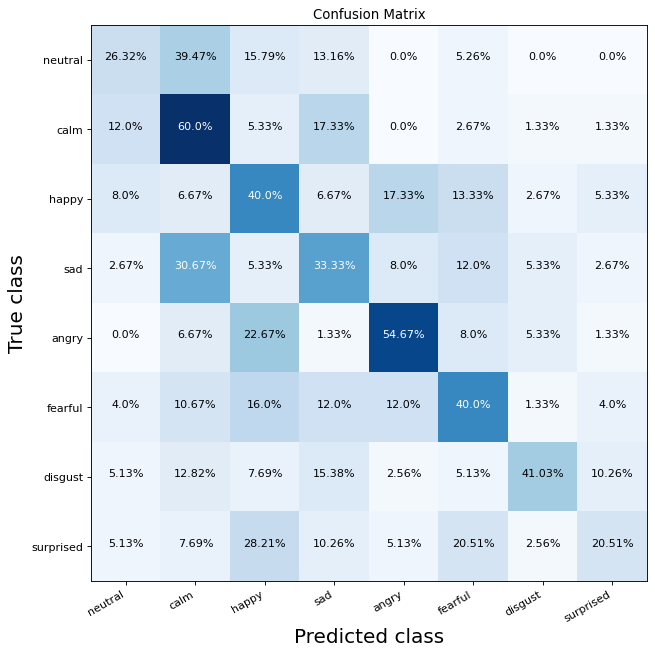
\includegraphics[width = 4in, keepaspectratio]{figures/CM_RAVDESS.png}
  \caption{Confusion matrix for RAVDESS dataset}
  \label{conf_matrix_rav}
\end{figure}

\begin{figure}[H]
  \centering
  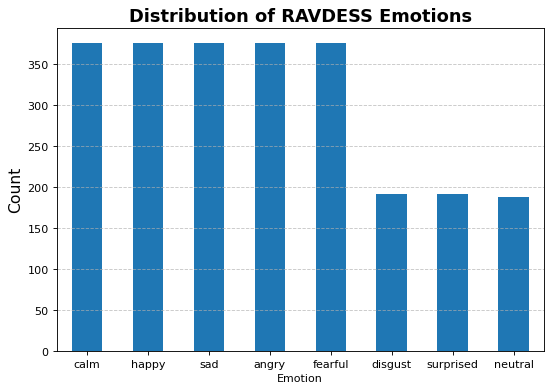
\includegraphics[width = 3in, keepaspectratio]{figures/Count Plot - RAVDESS.png}
  \caption{Distribution of classes for RAVDESS dataset}
  \label{dist_rav}
\end{figure}

The classification results for the RAVDESS dataset reveal varying levels of accuracy across different emotional classes. The emotions \textit{Calm} and \textit{Neutral} demonstrate moderate recognition accuracy, with \textit{Calm} achieving 60.0\% accuracy and \textit{Neutral} showing 26.32\%. However, \textit{Neutral} is frequently misclassified as \textit{Calm} (39.47\%) or other emotions, highlighting difficulties in distinguishing subtle emotional nuances. The emotion \textit{Angry} is relatively well-recognized, achieving 54.67\% accuracy, though it is occasionally confused with other high-arousal emotions such as \textit{Fearful} and \textit{Disgust}. Conversely, emotions like \textit{Surprised} and \textit{Sad} exhibit lower recognition accuracy, with \textit{Surprised} correctly identified only 20.51\% of the time, often being confused with \textit{Happy} and \textit{Fearful}. These findings suggest that the classifier struggles to accurately differentiate between emotions that exhibit subtle or overlapping features.

The results suggest that while the classifier is reasonably effective at identifying distinct high-arousal emotions like \textit{Angry}, it struggles with emotions that have subtle or overlapping features, such as \textit{Surprised} and \textit{Fearful}, \textit{Calm}, and \textit{Neutral}. Moreover, we expect in a biased scenario that the model would try to assign the most frequent labels for the least populated classes (\textit{Neutral, Disgust, Surprised}) but in general this was not observed here.

\section{Emo-DB}

The classification results for Emo-DB dataset can be seen in Table \ref{emo_results}. The total running time of the pipeline (training and testing) was about 3 minutes.

\begin{table}[h!]
\centering
\caption{Classification results ($\%$) over 10 random iterations - Emo-DB}
\begin{tabular}{lccccc}
\hline
 &  & Accuracy & Precision & Recall & F1 \\
\hline
\textbf{train} & Mean  & $49.6901$ & $48.2375$ & $49.6901$ & $47.9361$  \\
& Std   & $0.8321$ & $0.6664$ & $0.8321$ & $0.7483$  \\
\hline
\textbf{test}  & Top  & $53.271$   & $51.690$   & $50.782$   & -           \\
\hline
\label{emo_results}
\end{tabular}
\end{table}

The Emo-DB dataset's confusion matrix and class distribution for the testing set are shown in Figures \ref{conf_matrix_emo} and \ref{dist_emo}, respectively.

\begin{figure}[H]
  \centering
  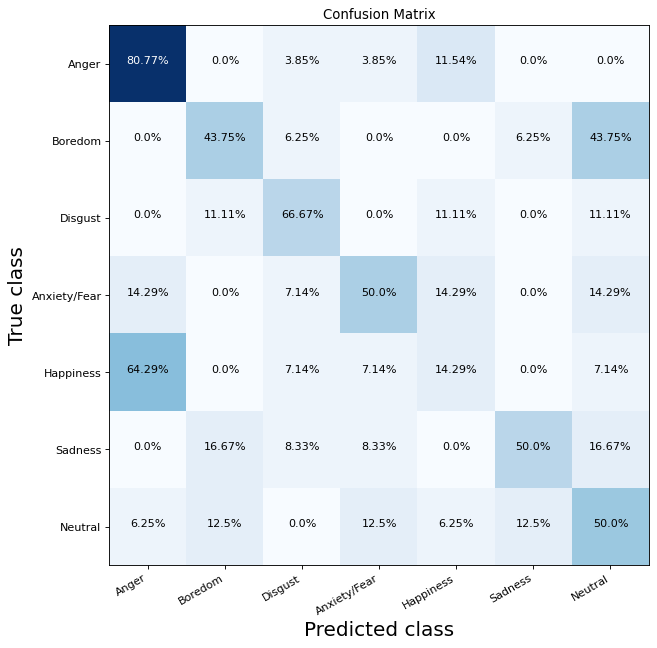
\includegraphics[width = 4in, keepaspectratio]{figures/CM_EMODB.png}
  \caption{Confusion matrix for Emo-DB}
  \label{conf_matrix_emo}
\end{figure}

\begin{figure}[H]
  \centering
  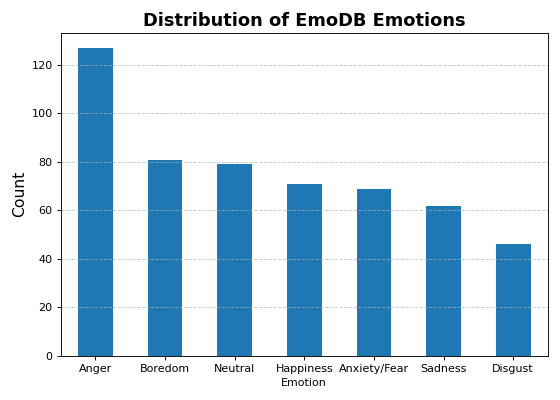
\includegraphics[width = 3in, keepaspectratio]{figures/Count plot - EmoDB.png}
  \caption{Distribution of classes for Emo-DB}
  \label{dist_emo}
\end{figure}

The emotion \textit{Anger} achieves high recognition accuracy, with 80.77\% of \textit{Anger} samples correctly classified. This aligns with the trend observed in the RAVDESS dataset, where high-arousal emotions are more easily identified. Additionally, \textit{Anger} is the majority class in this database, which may contribute to its higher classification performance. In contrast, lower recognition accuracy is observed for emotions such as \textit{Boredom} and \textit{Happiness}. For instance, \textit{Boredom} is correctly identified only 43.75\% of the time and is frequently misclassified as \textit{Neutral}. These results highlight the classifier's challenges in distinguishing lower-arousal or overlapping emotional states while excelling in recognizing dominant, high-arousal emotions.

These results highlight that high-arousal emotions such as \textit{Anger} are more readily distinguishable, while lower-arousal and subtle emotions like \textit{Neutral} and \textit{Boredom} are often misclassified, suggesting a need for feature enhancement or additional data to improve classification in these categories. There is also evidence of influence of the class distributions on the classification performance, as the model tends to misclassify emotions as the majority class \textit{Anger}.

\section{HAR}

The clasification results for HAR dataset can be seen in Table \ref{har_results}. The total running time of the pipeline (training and testing) was about 55 minutes.

\begin{table}[h!]
\centering
\caption{Classification results ($\%$) over 10 random iterations - HAR}
\begin{tabular}{lccccc}
\hline
 &  & Accuracy & Precision & Recall & F1 \\
\hline
\textbf{train} & Mean  & $95.9720$ & $95.9905$ & $95.9720$ & $95.9749$  \\
& Std   & $0.2461$ & $0.2474$ & $0.2461$ & $0.2465$  \\
\hline
\textbf{test}  & Top  & $93.247$   & $93.484$   & $93.524$   & -           \\
\hline
\label{har_results}
\end{tabular}
\end{table}

The confusion matrix for the HAR dataset, shown in Figure \ref{conf_matrix_har}, demonstrates strong classification performance across most activity classes. The class distribution, illustrated in Figure \ref{dist_har}, reveals a more balanced dataset, contributing to the overall high performance of the classifier.

\begin{figure}[H]
  \centering
  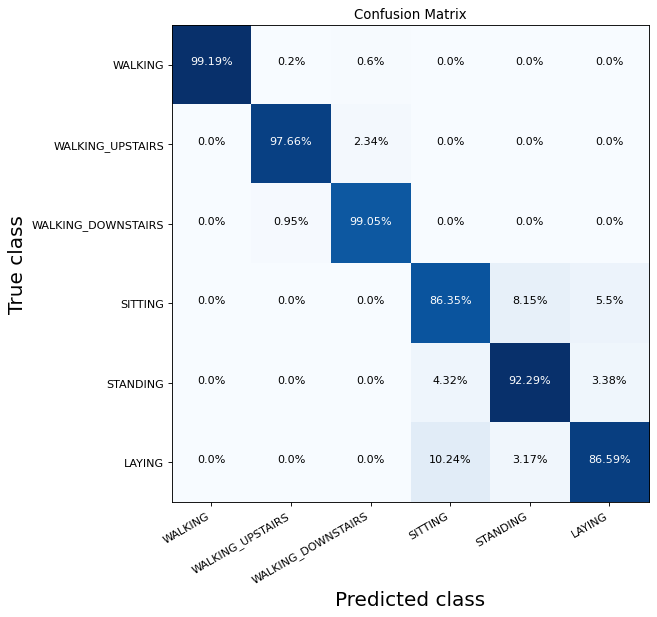
\includegraphics[width = 4in, keepaspectratio]{figures/CM_HAR.png}
  \caption{Confusion matrix for HAR dataset}
  \label{conf_matrix_har}
\end{figure}

\begin{figure}[H]
  \centering
  \includegraphics[width = 3in, keepaspectratio]{figures/Count Plot - HAR.png}
  \caption{Confusion Matrix for HAR dataset}
  \label{dist_har}
\end{figure}

The classifier exhibits excellent performance in identifying dynamic activities such as \textit{Walking}, with the \textit{Walking} and \textit{Walking\_Upstairs} classes achieving 99.19\% and 99.66\% accuracy, respectively. However, some confusion is observed between static activities like \textit{Standing} and \textit{Sitting}, with \textit{Sitting} being misclassified as \textit{Standing} in 8.15\% of cases, highlighting challenges in distinguishing between these similar postures. Additionally, while the activity \textit{Laying} is generally well-recognized, it has a 10.24\% misclassification rate with \textit{Sitting}, possibly due to overlapping features in body position. These results indicate that the classifier performs exceptionally well with dynamic activities but could benefit from further refinement in distinguishing static activities.

Overall, the classifier demonstrates high accuracy in recognizing dynamic activities (e.g., walking variations) but shows slight confusion between certain stationary activities, which could be an area for further optimization.

\section{Summary of results}

Across the three datasets, the classifier generally excels in recognizing dynamic activities and high-arousal emotions but encounters difficulties with classes that exhibit subtle distinctions or overlapping features. Dynamic activities, such as walking variations in the HAR dataset, and high-arousal emotions, such as anger in the Emo-DB and RAVDESS datasets, are consistently well-recognized. This is likely due to these classes possessing distinct and easily separable features, which the NVAR kernel can effectively capture.

In contrast, classes with subtle or overlapping features, such as static activities (e.g., sitting vs. standing) and low-arousal or nuanced emotions (e.g., calm vs. neutral, surprised vs. fearful), exhibit higher misclassification rates. These challenges reflect one of the limitations of the NVAR kernel—its heuristic-based approach to hyperparameter selection may not always yield optimal representations for complex or subtle classes, leading to suboptimal embeddings in such cases.

The results also indicate a noticeable tendency for the classifier to favor the majority class in each dataset, as observed with \textit{Anger} in the Emo-DB dataset. This suggests that the NVAR kernel may be sensitive to class imbalances, potentially due to its reliance on delay embeddings that may not fully account for unequal class distributions. To mitigate this bias towards more frequent classes, additional measures, such as improved class weighting or synthetic data augmentation, could be implemented.

Lastly, no significant differences were observed between training and testing set results, indicating that overfitting was not an issue during the training process. This consistency between the training and testing phases highlights the robustness of the implemented classification pipeline.
